
Recall that the notion of uniform relative stability (URS) in Definition \ref{def:URS} is the key to the necessary conditions for exact support recovery 
established in Theorem \ref{thm:necessary}.
In this chapter, we provide a complete characterization of the class of URS Gaussian arrays in terms of a simple condition on their covariance structure.
The condition is as follows.

% The proof of the main result is deferred until Section \ref{sec:proofs}.

% We define the class of dependence structures, referred to as uniformly decreasing dependence (UDD), for Gaussian arrays via their covariance matrices.

\begin{definition}[Uniformly decreasing dependence (UDD)] \label{def:UDD}
Consider a triangular array of jointly Gaussian distributed errors 
${\cal E} = \left\{\left(\epsilon_p(i)\right)_{i=1}^p, p = 1,2,\ldots\right\}$ 
with unit variances,
$$
\epsilon_p \sim \text{N}(0, \Sigma_p), \quad p=1,2,\ldots.
$$
The array ${\cal E}$ is said to be uniform decreasingly dependent (UDD) if 
for every $\delta>0$ there exists a finite $N(\delta)<\infty$, such that for every $i\in\{1,\ldots,p\}$, and $p\in\N$, we have
\begin{equation} \label{eq:UDD-definition}
    \Big|\left\{k\in\{1,\ldots,p\}:\Sigma_p(i,k)>\delta\right\}\Big| \le N(\delta)\quad \text{for all  } \delta>0.
\end{equation}
\end{definition}
That is, for every coordinate $i$, the number of elements which are more than $\delta$-correlated with $\epsilon_p(i)$ does not exceed $N(\delta)$. 

Note that the bound in \eqref{eq:UDD-definition} holds uniformly in $i$ and $p$, and only depends on $\delta$.
Also observe that on the left-hand side of \eqref{eq:UDD-definition}, we merely count in each row of $\Sigma_p$ the number of exceedances of covariances (not their absolute values!) over level $\delta$.

\begin{remark} \label{rmk:choice-of-N(delta)}
Without loss of generality, we may require that $N(\delta)$ be a monotone non-increasing function of $\delta$, for we can take
$$
N(\delta) = \sup_{p,i} \Big|\{k:\Sigma_p(i,k)>\delta\}\Big|,
$$
which is non-increasing in $\delta$.
Definition \ref{def:UDD} therefore states that the array is UDD when $N(\delta)<\infty$ for all $\delta>0$.
\end{remark}


Observe that the UDD condition does not depend on the order of the coordinates in the error 
vector $\epsilon_p = (\epsilon_p(i))_{i=1}^p$.  Often times, however, the errors are thought of 
coming from a stochastic process indexed by time or space.  To illustrate the generality of the 
UDD condition, we formulate next a simple sufficient condition (UDD$^\prime$) that is easier to 
check in a time-series context.

\begin{definition}[UDD\,$^\prime$]\label{d:UDD-prime}
For $\epsilon_p \sim \mathrm{N}(0,\Sigma_p)$ with unit variances, an array ${\cal E} = \left(\epsilon_p(i)\right)_{i=1}^p$ is said to satisfy the UDD\,$^\prime$ condition if there 
exist:
\begin{enumerate}
    \item[(i)] permutations $l_p$ of $\{1,\ldots,p\}$, for all $p\in\N$, and
    \item[(ii)] a non-negative sequence $(r_n)_{n=1}^\infty$ converging to zero $r_n\to 0$, as $n\to\infty$,
\end{enumerate}
such that 
\begin{equation} \label{eq:weak-correlation}
    \sup_{p\in\N} |\Sigma_p\left(i',j'\right)| \le r_{|i-j|}.
\end{equation}
where $i' = l_p(i)$, $j' = l_p(j)$, for all $i,j\in\{1,\ldots,p\}$.
\end{definition}

\begin{remark}
Without loss of generality, we may also require that $r_n$ be non-increasing in $n$, for we can replace $r_n$ with the non-increasing sequence $r'_n = \sup_{m\ge n} r_m$.
\end{remark}

\begin{proposition} \label{prop:UDD-equivalent}
UDD\,$^\prime$ implies UDD.
\end{proposition} 

\begin{proof}%[Proof of Proposition \ref{prop:UDD-equivalent}]
%The functions $N(\delta)$ and $r(n)=r_n$ are inverses of each other.
% {\bf $\text{UDD} \implies \text{UDD'}$:}
% If $N(0)<\infty$, then we can take 
% $$
% r_n = \underbrace{1, \ldots, 1}_{\lfloor N(0)/2\rfloor + 1}, 0, 0, \ldots.
% $$
% and recursively construct the permutations as follows.
% Start with any element

% We proof the contrapositive. 
% Suppose for all permutations and any sequence $r_n\to0$, there exists $i,j$ such that $\Sigma(i',j')>r_{|i'-j'|}$,
% then for any $\delta>0$ and any finite $M<\infty$, we can take $r_n$ to be a sequence of $M$ 1's followed by a $\delta$, i.e., 
% $$
% r_n = \underbrace{1, \ldots, 1}_{M+1}, \delta, \ldots.
% $$
% \fbox{Not true:}
% However, since there exists $i',j'$ such that $\Sigma(i',j')>r_{|i'-j'|}$, the set 
% $$
% S = l^{-1}\left(\left\{j',i'-N,\ldots,i'-1,i',i'+1,\ldots,i'+N\right\}\right)
% $$ 

% {\bf $\text{UDD'} \implies \text{UDD}$:} 
Since $r_n\to 0$, for any $\delta > 0$, there exists an integer 
$M = M(\delta)<\infty$ such that $r_n\le\delta$, for all $n\ge M$. 
Thus, by \eqref{eq:weak-correlation}, for every fixed 
$j' \in\{1,\ldots,p\}$, we can have $|\cov(\epsilon_p(k'),\epsilon_p(j'))| > \delta$,
only if $k'$ belongs to the set:
$$ 
 \left\{ k' \in \{1,\dots,p\} \, :\, j-M \le  k := l_p^{-1}(k') \le j+M \right\},
$$
where $j:= l_p^{-1}(j')$. That is, there are at most $2M+1<\infty$ indices  $k'\in\{1,\dots,p\}$, whose covariances with $\epsilon(j')$ may exceed $\delta$. 
Since this holds uniformly in $j'\in\{1,\ldots,p\}$, Condition UDD follows with 
$N(\delta) = 2M+1$.
\end{proof}



% \begin{definition}[Uniformly decreasing dependence (UDD)] \label{def:weak-dependence}
% Consider a triangular array of jointly Gaussian distributed errors $\left(\epsilon_p(j)\right)_{j=1}^p$ with unit variances, $\epsilon_p \sim \mathcal N(0,\Sigma_p)$. The array ${\cal E}$ is said to be uniform decreasingly dependent (UDD) with rate $(r_n)_{n=1}^\infty$ if 
% \begin{equation} \label{eq:weak-correlation}
%     \sup_p |\Sigma_p(i,j)| \le r_{|i-j|}
% \end{equation}
% such that $r_n\to 0$, as $n\to\infty$.
% \end{definition}
% 
% \begin{remark} \label{rmk:UDD-equivalent}
% In situations where there is no natural ordering of the components, it is sufficient that a permutation of the vector $\epsilon$ in its coordinates satisfy the requirements above. 
% In fact, the UDD condition can be equivalently stated as follows: for any $\delta>0$, and any coordinate $j\in\{1,\ldots,p\}$, there are at most $N(\delta)<\infty$ coordinates whose covariances with $\epsilon(j)$ exceed $\delta$; here $N(\delta)$ is a deterministic function independent of $p$.
% $N(\delta) \to 1$ as $\delta \to 0$.
% \end{remark}

We now state the main result of this chapter.  It states that a Gaussian array is URS if and only if it is UDD.
The URS condition essentially requires that the dependencies decay in a uniform fashion, the rate at which dependence decay 
does \emph{not} matter.

\begin{theorem} \label{thm:Gaussian-weak-dependence}
Let ${\cal E}$ be a Gaussian triangular array with standard normal marginals.  
The array ${\cal E}$ has uniformly relatively stable (URS) maxima if and only if it is uniformly decreasing dependent (UDD).
\end{theorem}

% The proof of Theorem \ref{thm:Gaussian-weak-dependence} is given in Section \ref{sec:proofs}. 

Specifically, for stationary Gaussian arrays, we have the following corollary.

\begin{corollary} \label{cor:stationary-Gaussian-errors}
Let ${\cal E} = \{\epsilon_p(i) = Z(i)\}$ for a stationary Gaussian time series ${\cal Z} = \{Z(i)\}$.
Then $\cal E$ is {URS} if and only if the autocovariance function $\cov(Z(k), Z(0))\to 0$, as $k\to\infty$.
\end{corollary}

Corollary \ref{cor:stationary-Gaussian-errors} follows by Theorem \ref{thm:Gaussian-weak-dependence} and the observation that UDD is equivalent to vanishing autocovariance of $\cal Z$.
A slightly weaker form of the ``if'' part was established in Theorem 3 of \cite{berman1964limit}.

Returning again to the study of support recovery problems, Theorem \ref{thm:Gaussian-weak-dependence} and the necessary condition for exact support recovery in Theorem \ref{thm:necessary} yield the following result.

\begin{corollary} \label{cor:weakly-dependent-errors}
For UDD Gaussian errors, the result in Theorem \ref{thm:necessary} holds.
\end{corollary}

One may ask, whether the UDD (equivalently, URS) condition can be relaxed further for the phase-transition result in Theorem \ref{thm:necessary} to 
hold.  As a counterpart to Remark \ref{rmk:dependence-assumptions}, we demonstrate next that the dependence conditions in Theorem \ref{thm:necessary} 
are nearly optimal.  Specifically, we show that if the URS dependence condition is violated, then it may be possible to recover the support 
of weaker signals, falling below the boundary.   The main idea is to use the equivalence of URS and UDD to construct a Gaussian error array,
whose correlations do not decay in a uniform fashion (UDD fails). As we will see, in such a case one can do substantially better in terms of 
support recovery.  This shows that the URS condition is nearly optimal in the Gaussian setting.  
Numerical simulations illustrating this example can be found in Section \ref{suppsec:numerical}, below. 

\begin{example}[On the tightness of the URS condition for exact support recovery] \label{exmp:counter-example}
Suppose ${\cal E} = \left(\epsilon_p(i)\right)_{i=1}^p$ is Gaussian, and is comprised of $\lfloor p^{1-\beta}\rfloor$ blocks, each of size at least $\lfloor p^\beta \rfloor$.  Let the elements within each block have correlation 1, and let the elements from different blocks be independent. 
If $\underline{r} \ge 4(1-\beta)$, then the procedure 
$$
 \widehat{S} = \big\{i:x(i)>\sqrt{2(1-\beta)\log{p}}\big\}
 $$ 
yields exact support recovery, i.e., $\mathbb P[\widehat{S} = S] \to 1$, as $p\to\infty$.  This requirement on the signal size is strictly 
weaker than that of the strong classification boundary, since $4(1-\beta) < (1 + \sqrt{1-\beta})^2$ on $\beta\in(0,1)$.
\end{example} 
\begin{proof}[Example \ref{exmp:counter-example}]
Let $t_p^* = \sqrt{2(1-\beta)\log{p}}$  and observe that $\widehat{S} = \{j:x(j)>t_p^*\}$.
Analogous to \eqref{eq:Bonferroni-FWER-control} in the proof of Theorem \ref{thm:sufficient}, we have
\begin{align*}
    \P\left[\widehat{S} \subseteq S\right] 
        &= 1 - \P\left[\max_{j\in S^c}x(j) > t_p^*\right] 
        = 1 - \P\left[\max_{j\in S^c}\epsilon(j) > t_p^*\right] \nonumber \\
      % \ge 1 - \P\left[\max_{j\in\{1,\ldots,p\}}\epsilon(j) > t_p\right] \nonumber \\
        &\ge 1 - \P\left[\max_{j\in\{1,\ldots,p\}}\epsilon(j) > t_p^*\right] 
        \ge 1 - \P\left[\max_{j\in\{1,\ldots,\lfloor p^{1-\beta}\rfloor\}}\widetilde{\epsilon}(j) > t_p^*\right]
\end{align*}
where $\left(\widetilde{\epsilon}\right)_{j=1}^{\lfloor p^{1-\beta}\rfloor}$'s are independent Gaussian errors; in the last inequality we used the assumption that there are at most $\lfloor p^{1-\beta}\rfloor$ independently distributed Gaussian errors in $\left(\epsilon_p(j)\right)_{j=1}^p$.
By Example \ref{exmp:FWER-controlling_procedures} (with $\lfloor p^{1-\beta}\rfloor$ taking the role of $p$), we know that the FWER goes to 0 at a rate of 
$\left(2\log{\lfloor p^{1-\beta}\rfloor}\right)^{-1/2}$.
Therefore, the probability of no false inclusion converges to 1.


On the other hand, since the signal sizes are no smaller than $(\nu\underline{r}\log p)^{1/\nu} = \sqrt{2\underline{r}\log p}$ (for $\nu = 2$), similar to 
\eqref{eq:sufficient-proof-eq1}, we obtain
\begin{align}
    \P\left[\widehat{S} \supseteq S\right] 
    &\ge \P\left[\min_{j\in S}\epsilon(j) > \sqrt{2(1-\beta)\log{p}} - \sqrt{2\underline{r}\log{p}} \right] \nonumber \\
    &= \P\left[\max_{j\in S}\left(-\epsilon(j)\right) < \sqrt{2\log{p}}\left(\sqrt{\underline{r}}-\sqrt{1-\beta}\right) \right] \nonumber \\
    &= \P\left[\frac{\max_{j\in S}(-\epsilon(j))}{u_{|S|}} < \frac{\sqrt{\underline{r}}-\sqrt{1-\beta}}{\sqrt{1-\beta}}\left(1+o(1)\right) \right], \label{eq:sufficient-proof-counter-example}
\end{align}
where in the last line we used the quantiles \eqref{eq:AGG-quantiles}.
Since the minimum signal size is bounded below by $\underline{r} > 4(1-\beta)$, the right-hand-side of the inequality in \eqref{eq:sufficient-proof-counter-example} converges to a constant strictly larger than 1. While the left-hand-side, by Slepian's lemma (recall 
Theorem \ref{thm:Slepian-lemma} and Relation \ref{e:Slepian-lemma-maxima}), is stochastically smaller than a r.v.\ going to 1.  Namely, we have
\begin{equation}
  \frac{1}{u_{|S|}} \max_{j\in S}(-\epsilon(j)) \stackrel{d}{\le} \frac{1}{u_{|S|}} \max_{j\in S} \epsilon^*(j) \stackrel{\P}{\longrightarrow} 1,
\end{equation}
where $\left({\epsilon^*}\right)_{j=1}^{\lfloor p^{1-\beta}\rfloor}$'s are independent Gaussian errors.
Therefore the probability in \eqref{eq:sufficient-proof-counter-example} must also converge to 1.
\end{proof}




\medskip

Before proceeding to the proof of Theorem \ref{thm:Gaussian-weak-dependence}, we will briefly discuss 
the relationships between UDD and other dependence conditions in the context of extreme value theory. The main idea
we would like to convey is that UDD (and equivalently URS) is an exceptionally mild condition on the dependence of the array.

\medskip
\noindent{\bf The Berman and UDD conditions.} 
 \label{UDD_and_Berman}
 Suppose that the array of errors  ${\cal E}$ comes from a stationary Gaussian time series $\epsilon(i),\ i\in \mathbb{N}$, with auto-covariance $r_p=\cov(\epsilon(i+p),\epsilon(i))$. 
One is interested in the asymptotic behavior of the maxima $M_p:=\max_{i=1,\dots,p} \epsilon(i)$.

In this setting, the Berman's condition, introduced in \cite{berman1964limit}, requires that
\begin{equation} \label{eq:Berman}
    r_p \log p \to 0,\ \ \mbox{ as }p\to\infty.
\end{equation}
This condition entails that 
\begin{equation}
    \label{eq:Gauss-max-in-distribution}
  a_p (M_p - b_p) \stackrel{d}{\longrightarrow } Z,\  \ \mbox{ as }p\to\infty,
\end{equation}
with the Gumbel limit distribution $\mathbb P [Z\le x] = \exp\{-e^{-x}\},\ x\in \mathbb R$, 
where 
$$
a_p = \sqrt{2\log p},\quad b_p  = \sqrt{2\log p} - \frac{1}{2}\left(\sqrt{2\log p}\right)^{-1}\left(\log \log (p) + \log(4\pi)\right),
$$ 
are {\em the same} centering and normalization sequences
as in the case of iid $\epsilon(i)$'s.  
Berman's condition is one of the weakest dependence conditions  in the literature for which the convergence in \eqref{eq:Gauss-max-in-distribution} holds. 
See, e.g., Theorem 4.4.8 in \cite{embrechts2013modelling}, where \eqref{eq:Berman} is described as ``very weak''.

Instances where the dependence in the time series is so strong that Berman's condition \eqref{eq:Berman} fails have also been studied.  In such 
cases, one may continue to have \eqref{eq:Gauss-max-in-distribution} but typically the sequences of normalizing and centering constants will be
{\em different} from the iid case, and the corresponding limit is usually no longer Gumbel; see, for example, Theorems 6.5.1 and  6.6.4 in \cite{leadbetter2012extremes}, and \cite{mccormick1976weak}. 
% In particular, \cite{mccormick1976weak} derived the normalizing constants when both $r_p\to 0$ monotonically and  $r_p \log p \to \infty$ monotonically, as $p\to\infty$. 
% In this case, convergence in distribution still takes place, with the maxima concentrating along a sequence asymptotic to \eqref{eq:quantiles}.

In our high dimensional support estimation context, the notion of relative stability is sufficient and more natural than the finer notions of distributional convergence.
If one is merely interested in the asymptotic relative stability of the Gaussian maxima, then Berman's condition can be relaxed significantly 
\citep[see also, Theorem 4.1 of][]{berman1964limit}.  Observe that by Proposition \ref{prop:UDD-equivalent},  the Berman condition \eqref{eq:Berman} implies UDD and hence relative stability (Theorem \ref{thm:Gaussian-weak-dependence}), i.e., 
\begin{equation} \label{eq:Gaussian-URS}
  \frac{1}{b_p} M_p \stackrel{\mathbb P}{\to} 1,\quad\mbox{as}\quad p\to\infty.
\end{equation}
This {\em concentration of maxima} property can be readily deduced from \eqref{eq:Gauss-max-in-distribution}, since $a_p b_p \sim 2\log(p) \to \infty$ as $p\to\infty$.
Theorem \ref{thm:Gaussian-weak-dependence} shows that \eqref{eq:Gaussian-URS} holds if the much weaker uniform dependence condition UDD holds. 
Note that our condition is coordinate free --- neither monotonicity of the sequence $r_p$ nor stationarity of the underlying array is required. This
makes it substantially broader than the time series setting in the seminal work \cite{berman1964limit}.

% The method of proof is also very different from the results on distributional convergence in the references mentioned above. 

\medskip

The rest of this chapter is devoted to the proof of the main result, i.e., Theorem \ref{thm:Gaussian-weak-dependence}. 
We first introduce a key lemma regarding the structure of an {\em arbitrary} correlation matrix of high-dimensional random variables.
The proof uses a surprising, yet elegant application of Ramsey's Theorem from the study of combinatorics.
%; this application, and its consequences in high-dimensional probability, are presented in Section \ref{subsec:Ramsey}.
The `only if' part of Theorem \ref{thm:Gaussian-weak-dependence} follows from this lemma, in Section \ref{sec:URS=>UDD}. 

The proof of the `if' part is detailed in Section \ref{sec:UDD=>URS}.
The arguments there have been recently extended to establish bounds on the rate of concentration of maxima in \cite{kartsioukas2019rate}; see also, \cite{tanguy2015some} and the related notion of super-concentration of \cite{chatterjee2014superconcentration}.

\section{Ramsey's  theory and the structure of correlation matrices} 
\label{sec:Ramsey}


% We start by providing a general result on the structure of arbitrary correlation matrices in this section, which helps us establish the `only if' part of Theorem \ref{thm:Gaussian-weak-dependence}. 
% Its proof uses the Ramsey Theorem from graph theory, which we briefly review next.

Given any integer $k\ge 1$, there is always an integer $R(k,k)$ called the {\em Ramsey number}:
\begin{equation}\label{eq:Ramsey-number}
k\le R(k,k)\le \binom{2k-2}{k-1}
\end{equation}
such that the following property holds:
every undirected graph with at least $R(k,k)$ vertices will contain {\em either} a clique of size $k$, or an {\em independent set} of $k$ nodes. 
Recall that a clique is a complete sub-graph where all pairs of nodes are connected, and an independent set is a set of nodes where no two nodes are connected.

This result is a consequence of the celebrated work of \citet{ramsey2009problem}, which 
gave birth to Ramsey Theory \citep[see e.g.,][]{conlon2015recent}.  
The Ramsey Theorem and the upper bound \eqref{eq:Ramsey-number} \citep[established first in][]{erdos1935combinatorial} are at the heart of the proof of the following result.  A recent improvement on the upper bound is given by \cite{sah:2020}.
%An excellent introduction to Ramsey theory is given in \url{http://math.mit.edu/~fox/MAT307-lecture05.pdf}. 

\begin{proposition} \label{prop:lower-bound-correlation-Ramsey}
  Fix $\gamma\in(0,1)$ and let $P = \left(\rho(i,j)\right)_{n\times n}$ be an arbitrary correlation
  matrix. If 
  \begin{equation}\label{eq:Ramsey-the-k-def}
   k:= \lfloor \log_2({n})/2 \rfloor  \ge \lceil 1/\gamma \rceil + 1,
  \end{equation}
  then there is a set of $k$ indices $K = \{l_1, \ldots, l_k\}\subseteq \{1,\ldots,n\}$ 
  such that 
  \begin{equation} \label{eq:lower-bound-correlation-Ramsey}
      \rho(i,j) \ge -\gamma, \mbox{ for all } i,j\in K.
  \end{equation}
\end{proposition}

\begin{proof}%[Proof of Proposition \ref{prop:lower-bound-correlation-Ramsey}]
By using \eqref{eq:Ramsey-number} and a refinement of the Stirling's formula, 
we will show at the end of the proof that for $k \le \log_2({n})/2$, we have 
\begin{equation}\label{eq:Ramsey-bounds}
 R(k,k) \le n,
\end{equation}
where $R(k,k)$ is the Ramsey number.  

Now, construct a graph with vertices $\{1,\dots,n\}$ such that there is an edge between nodes $i$ and $j$ if and only if $\rho(i,j) \ge -\gamma$. 
In view of \eqref{eq:Ramsey-bounds} and Ramsey's theorem (see e.g., Theorem 1 in \cite{fox2009lecture} or \cite{conlon2015recent} for a recent survey on Ramsey theory), there is a subset of $k$ nodes $K =\{l_1,\dots,l_k\}$, which is either a {\em complete graph} or an {\em independent set}.  Recall that in a
complete graph, every two nodes are connected with an edge; while in independent sets, no two nodes are connected.

If $K$ is a complete graph, then by our construction of the graph, Relation \eqref{eq:lower-bound-correlation-Ramsey} holds. 

Now, suppose that $K$ is a set of independent nodes.  This means, again by the construction of our graph, that
$$
\rho(i,j) < -\gamma,\quad\mbox{for all }i\not= j\in K.
$$
Let $Z_i,\ i \in K$ be zero-mean random variables such that 
$\rho(i,j) = \E [Z_iZ_j]$. Observe that
\begin{equation} \label{eq:Ramsey-proof-contradiction}
    \var\left( \sum_{i\in K} Z_i\right) 
    = \sum_{i\in K} \var(Z_i) + \sum_{\substack{i\not=j\\i,j \in K}} \cov(Z_i, Z_j) 
    <  k - k(k-1)\gamma,
\end{equation}
since $\var(Z_i)=1$ and $\rho(i,j)<-\gamma$ for $i\neq j$.
By our assumption, $k\ge \left(\lceil 1/\gamma \rceil + 1\right)$, or equivalently, $(k-1) \ge 1/\gamma$, the variance in \eqref{eq:Ramsey-proof-contradiction} is negative. 
This is a contradiction showing that there are no independent sets $K$ with cardinality $k$.

To complete the proof, it remains to show that Relation \eqref{eq:Ramsey-bounds} holds.
In view of the upper bound on the Ramsey numbers \eqref{eq:Ramsey-number}, it 
is enough to show that $k \le \log_2(\sqrt{n})$ implies
$$
\binom{2k-2}{k-1} \le n.
$$
This follows from a refinement of the Stirling formula, due to \citet{robbins1955remark}:
$$
 \sqrt{2\pi} m^{m+1/2} e^{-m} e^{\frac{1}{(12 m +1)}} \le  m! \le \sqrt{2\pi} m^{m+1/2} e^{-m} 
 e^{\frac{1}{12 m}}.
$$
Indeed, letting $\widetilde k:= k-1$, and applying the above upper and lower bounds 
to the  terms $(2\widetilde k)!$ and $\widetilde k!$, respectively, we obtain:
\begin{align*}
\binom{2k-2}{k-1} \equiv \frac{(2\widetilde k)!}{ (\widetilde k!)^2 }
\le \frac{2^{2\widetilde k}}{\sqrt{\pi \widetilde k}}\exp\left \{ \frac{1}{24 \widetilde k} -
\frac{2}{ 12 \widetilde k +1}\right\} < 2^{2 k}
\end{align*}
where the last two inequalities follow by simply dropping positive factors less than $1$.
Since $2k \le \log_2(n)$, the above bound implies Relation \eqref{eq:Ramsey-bounds} 
and the proof is complete.
\end{proof}

Using Proposition \ref{prop:lower-bound-correlation-Ramsey}, we establish the key lemma used in the proof of Theorem \ref{thm:Gaussian-weak-dependence}.


\begin{lemma} \label{lemma:positive-correlation}
  Let $c\in(0,1)$, and $P = \left(\rho(i,j)\right)_{(n+1)\times(n+1)}$ be a correlation matrix such that \begin{equation} \label{eq:positive-correlation-lemma-condition}
      \rho(1,j) > c \quad \mbox{for all } j = 1,\ldots,n+1.
  \end{equation}
  If $n \ge 2^{2\lceil2/c^2\rceil+4}$, then there is a set of indices $K = \{l_1, \ldots, l_k\}\subseteq \{2,\ldots,n+1\}$ of cardinality $k = |K| = \lfloor\log_2{\sqrt{n}}\rfloor$, such that 
  \begin{equation} \label{eq:positive-correltation-lemma-conclusion}
      \rho(i,j) > \frac{c^2}{2} \quad\mbox{for all } i,j\in K.
  \end{equation}
  That is, all entries of the $k\times k$ sub-correlation matrix $P_K:=\left(\rho(i,j)\right)_{i,j\in K}$ are larger than $c^2/2$.
\end{lemma}

\begin{proof}[Lemma \ref{lemma:positive-correlation}]
    Let $Z_1, \ldots, Z_{n+1}$ be random variables with covariance matrix $P$.
    Denote $\rho_j = \rho(1,j)$ and define 
    \begin{equation}
      R_j = 
      \begin{cases}
        \frac{1}{\sqrt{1-\rho_j^2}}\left(Z_j - \rho_j Z_1\right), &\mbox{if } \rho_j<1,\\
        R^* &\mbox{if } \rho_j=1,
      \end{cases}
    \end{equation}
    where $R^*$ is an arbitrary zero-mean, unit-variance random variable.
    It is easy to see that $\var(R_j) = 1$, and
    \begin{align*}
    \cov\left(Z_i, Z_j\right) &= \cov\left(\rho_i Z_1 + \sqrt{1-\rho_i^2} R_i, \; \rho_j Z_1 + \sqrt{1-\rho_j^2} R_j\right) \\
        &= \rho_i\rho_j + \sqrt{1-\rho_i^2}\sqrt{1-\rho_j^2} \;\cov\left(R_i, R_j\right) \\
        &> c^2 + \min\left\{\cov\left(R_i, R_j\right), 0\right\}.
    \end{align*}
    
    Therefore, Relation \eqref{eq:positive-correltation-lemma-conclusion} would hold if we can find a set of indices $K = \{l_1,\ldots,l_k\}$ such that $\cov\left(R_i,R_j\right)\ge -c^2/2$ for all $i,j\in K$, where $k=|K|=\lfloor\log_2\sqrt{n}\rfloor$.
    This, however, follows from Proposition \ref{prop:lower-bound-correlation-Ramsey} applied to $\left(R_j\right)_{j=2}^{n+1}$ with $\gamma = c^2/2$, provided that 
    $$
    k = \lfloor\log_2\sqrt{n}\rfloor \ge \lceil 2/c^2 \rceil + 1.
    $$
    The last inequality indeed follows form the assumption that $n \ge 2^{2\lceil2/c^2\rceil+4}$.
\end{proof}




\section{URS implies UDD (Proof of the `only if' part of Theorem \ref{thm:Gaussian-weak-dependence})} 
\label{sec:URS=>UDD}

In view of Remark \ref{rmk:choice-of-N(delta)}, UDD is equivalent to the requirement that
$N(\delta) := 1+\sup_{p} N_p(\delta) < \infty$ for all $\delta\in(0,1)$,
where 
\begin{equation} \label{eq:N_p(c)}
    N_p(\delta) := \max_{j\in\{1,\ldots,p\}} \Big|\{i:i\neq j,\;\Sigma_p(j,i) > \delta\}\Big|.
\end{equation}
Therefore, if ${\cal E}$ is not UDD, then there must exist a constant $c\in (0,1)$ for which $N(c)$ is infinite, i.e., there is a subsequence $\widetilde p\to\infty$ such that $N_{\widetilde p}(c) \to \infty$.
Without loss of generality,  we may assume that $\widetilde{p}=p$.

Let $j_p(c)$ be the maximizers of \eqref{eq:N_p(c)}, and let
\begin{equation} \label{eq:sub-sequence_of_sets}
S_p(c):= \{ i\in\{1,\dots,p\}\, :\, \Sigma_p(j_p(c), i) > c \}.% \quad\quad \text{for all }k\in S_p(c).
\end{equation}
Observe that $|S_p(c)| = N_p(c)+1 \to \infty$, as $p\to\infty$ 
(note $j_p(c) \in S_{p}(c)$).

Applying Lemma \ref{lemma:positive-correlation} to the set of random variables indexed by $S_p(c)$, we conclude, for $N_p(c) \ge 2^{2\lceil2/c^2\rceil+4}$, there must be a further subset 
\begin{equation} \label{eq:further_sub-sequence_of_sets}
  K_p(c) \subseteq S_p(c),
\end{equation}
of cardinality 
\begin{equation} \label{eq:further_sub-sequence_of_sets_size}
k_p(c) := \left|K_p(c)\right| \ge \log_2{\sqrt{N_p(c)}},
\end{equation}
such that all pairwise correlations of the random variables indexed by $K_p(c)$ are greater than $c^2/2$.
Since the sequence $N_p(c)\to\infty$, by \eqref{eq:further_sub-sequence_of_sets_size}, we have $k_p(c)\to\infty$ as $p\to\infty$.

Therefore, we have identified a sequence of subsets $K_p(c)\subseteq\{1,\ldots,p\}$ with the following two properties:
\begin{enumerate}
  \item $k_p(c) := \left|K_p(c)\right| \to \infty$, as $p\to\infty$, and
  \item For all $i,j\in K_p(c)$, we have
  \begin{equation} \label{eq:further_sub-sequence_of_sets_cor}
    \Sigma_p(i,j) > c^2/2.
  \end{equation}
\end{enumerate}
Without loss of generality, we may assume $K_p(c) = \{1,\ldots,k_p(c)\} \subseteq \{1,\ldots,p\}$, upon re-labeling of the coordinates. 

Now consider a Gaussian sequence $\epsilon^* = \{\epsilon^*(j),\;j = 1,2,\ldots\}$, independent of ${\cal E}$, defined as follows:
$$
\epsilon^*(j):= Z \left(c/\sqrt{2}\right) + Z(j) \sqrt{1-{c^2}/{2}}, \quad j = 1, 2, \ldots,
$$ 
where $Z$ and $Z(j), j = 1, 2, \ldots$ are independent standard normal random variables. 
Hence,
\begin{equation} \label{eq:Slepian-conclusion-condition-1}
    {\rm Var}(\epsilon^*(j)) = 1 = {\rm Var}(\epsilon_p(j)),
\end{equation}
and
\begin{equation} \label{eq:Slepian-conclusion-condition-2}
    \cov(\epsilon^*(i),\epsilon^*(j)) = \frac{c^2}{2} \le \cov(\epsilon_p(i),\epsilon_p(j)),
\end{equation}
for all $p$, and all $i\neq j$, $i,j\in K_p(c)$.
Thus we have, as $p\to\infty$, 
\begin{equation} \label{eq:!UDD=>subsequence-fail}
    \frac{1}{u_{k_p(c)}} \max_{j\in K_p(c)} \epsilon^*(j) = \frac{c/\sqrt{2}}{u_{k_p(c)}}Z + \frac{\sqrt{1-c^2/2}}{u_{k_p(c)}} \max_{j\in K_p(c)} Z(j) \stackrel{\mathbb P}{\to} \sqrt{1-\frac{c^2}{2}},
\end{equation}
where the convergence in probability follows from Proposition \ref{prop:rapid-varying-tails} part \ref{prop:rapid-varying-tails_part-ii}.
%The fact that the last limit is strictly less than $1$, together with Relation \eqref{eq:Slepian-conclusion}, shows that \eqref{eq:URS-condition} is impossible, for $S_p:=K_p(c)$.

Relations \eqref{eq:Slepian-conclusion-condition-1} and \eqref{eq:Slepian-conclusion-condition-2}, by Slepian's Lemma (recall
Theorem \ref{thm:Slepian-lemma}), also imply,
\begin{equation}\label{eq:Slepian-conclusion}
  \frac{1}{u_{k_p(c)}} \max_{j\in K_p(c)} \epsilon^*(j) \stackrel{d}{\ge} \frac{1}{u_{k_p(c)}} \max_{j\in K_p(c)} \epsilon_p(j).
\end{equation}
Therefore, by \eqref{eq:Slepian-conclusion} and \eqref{eq:!UDD=>subsequence-fail}, for all $\sqrt{1-c^2/2} \le \delta < 1$, we have,
$$
\P\left[\frac{1}{u_{k_p(c)}} \max_{j\in K_p(c)} \epsilon_p(j) < \delta \right] \to 1 \quad\mbox{as  }p\to\infty.
$$
This contradicts the definition of URS (with the particular choice of $S_p:=K_p(c)$), and the proof of the `only if' part of 
Theorem \ref{thm:Gaussian-weak-dependence} is complete.



\section{UDD implies URS (Proof of the `if' part of Theorem \ref{thm:Gaussian-weak-dependence})} 
\label{sec:UDD=>URS}

Recall that our objective is to show \eqref{eq:URS-condition}. 
We will do so in two stages; namely, we will prove that for all $\delta>0$, we have 
\begin{equation} \label{eq:URS-condition-upper-side}
    \P\left[\frac{M_{S_p}}{u_{|S_p|}} > 1+\delta\right] \to 0,
\end{equation}
and
\begin{equation} \label{eq:URS-condition-lower-side}
    \P\left[\frac{M_{S_p}}{u_{|S_p|}} < 1-\delta\right] \to 0,
\end{equation}
for any sequence of subsets $S_p$ such that $|S_p|\to\infty$.
Although the first step \eqref{eq:URS-condition-upper-side} was already shown in Proposition \ref{prop:rapid-varying-tails}, regardless of the dependence structure, we provide in this section a more refined result. 
Specifically, the following result states that for the AGG model, the constant $\delta$ in Proposition \ref{prop:rapid-varying-tails} can be replaced by a vanishing sequence $c_p\to 0$.

\begin{lemma}[Upper tails of AGG maxima] \label{lemma:AGG-maxima-upper-tails}
Let ${\cal E}$ be an array with marginal distribution $F\in\text{AGG}(\nu)$, $\nu>0$. If we pick
\begin{equation} \label{eq:choice-of-c_p}
    c_p = \frac{u_{p\log{p}}}{u_p} - 1,    
\end{equation} 
where $u_p = F^{\leftarrow}(1-1/p)$, then we have $c_p>0$, $c_p\to 0$, and
\begin{equation} \label{eq:AGG-max-upper-bound}
    \P\left[\frac{M_p}{u_p}-(1+c_p) > 0\right] \to 0.
\end{equation}
\end{lemma}
The proof can be found in Section \ref{subsec:bounding-upper-tails-of-maxima} below.

Since Lemma \ref{lemma:AGG-maxima-upper-tails} holds regardless of the dependence structure, the same conclusions hold if one replaces $M_p$ by $M_{S_p} = \max_{j\in S_p}\epsilon(j)$ and $p$ by $q = q(p)=|S_p|$, where $S_p$ is any sequence of sets such that $q \equiv |S_p| \to \infty$.
This entails \eqref{eq:URS-condition-upper-side}.

On the other hand, the proof of \eqref{eq:URS-condition-lower-side} uses a more elaborate argument based on the Sudakov-Fernique bound.
We proceed by first bounding the probability by an expectation. 
For all $\delta>0$, we have
\begin{align}
    \P\left[\frac{M_{S_p}}{u_q}<1-\delta\right] 
        &= \P\left[-\left(\frac{M_{S_p}}{u_q} - (1+c_q)\right) > \delta + c_q\right] \nonumber \\
        %&\le \P\left[\max{\left\{-\left(\frac{M_{S_p}}{u_q} - (1+c_q)\right),0\right\}} > \delta + c_q\right] \nonumber \\
        &\le \P\left[\left(\frac{M_{S_p}}{u_q} - (1+c_q)\right)_->\delta+c_q\right] \nonumber \\
        &\le \frac{1}{\delta + c_q}\E\left[\left(\frac{M_{S_p}}{u_q} - (1+c_q)\right)_-\right], \label{eq:Gaussian-maxima-lower-expectation-bound}
\end{align}
where $(x)_-:=\max\{-x,0\}$ and the last line follows from the Markov inequality.
The next result shows that the upper bound in \eqref{eq:Gaussian-maxima-lower-expectation-bound} vanishes.
\begin{lemma} \label{lemma:Gaussian-maxima-lower-expectation}
  Let ${\cal E}$ be a Gaussian UDD  array  and 
  $S_p\subseteq\{1,\ldots,p\}$ be an arbitrary sequence of sets 
  such that $q = q(p) = |S_p|\to\infty$.  Then, for $M_{S_p}:= \max_{j\in S_p} \epsilon_p(j)$ and $c_q$ as in \eqref{eq:choice-of-c_p}, we have
  \begin{equation} \label{eq:Gaussian-maxima-lower-expectation}
    \E\left[\left(\frac{M_{S_p}}{u_q} - (1+c_q)\right)_-\right] \to 0,\ \ \quad \mbox{ as }p\to \infty.
  \end{equation}
\end{lemma}
The proof of the lemma is given in Section \ref{subsec:bounding-lower-tails-of-maxima} below.


Going back to the proof of Theorem \ref{thm:Gaussian-weak-dependence}, we observe that Relations \eqref{eq:Gaussian-maxima-lower-expectation-bound} and \eqref{eq:Gaussian-maxima-lower-expectation} imply \eqref{eq:URS-condition-lower-side}, which completes the proof of the `if' part of
Theorem \ref{thm:Gaussian-weak-dependence}. \qed 

\begin{remark} Only the Sudakov-Fernique minorization argument used in the proof of Lemma \ref{lemma:Gaussian-maxima-lower-expectation}, relies on the Gaussian assumption. We expect the techniques and results here to be useful in extending Theorem \ref{thm:Gaussian-weak-dependence} to more general class of distributions, say, the AGG model.
\end{remark}


\subsection{Bounding the upper tails of AGG maxima}
\label{subsec:bounding-upper-tails-of-maxima}


\begin{proof}[Lemma \ref{lemma:AGG-maxima-upper-tails}]
Recall by \eqref{eq:AGG-quantiles} that 
\begin{equation*}
    u_q\sim\left(\nu\log{q}\right)^{1/\nu}, \quad q\to\infty,
\end{equation*}
so that
\begin{equation} %\label{eq:choice-of-c_p}
c_p  = \frac{u_{p\log{p}}}{u_p} -1 = \left(\frac{\log{p}+\log{\log{p}}}{\log{p}}\right)^{1/\nu}(1+o(1)) - 1 \rightarrow 0 \quad \mbox{as } p\to\infty.
\end{equation} 
By the union bound, we have
\begin{align}
    \P\left[\frac{M_p}{u_p} > 1+c_p\right] 
        &\le \sum_{j=1}^p \P\left[\frac{\epsilon_p(j)}{u_p} > 1+c_p\right] 
        = p \overline{F}\left(u_{p\log{p}}\right) \label{eq:AGG-maxima-upper-tails-proof-1} \\
        &= p \overline{F}\left(F^{\leftarrow}\left(1-\frac{1}{p\log{p}}\right)\right) \le \frac{1}{\log{p}} \rightarrow 0. \nonumber
\end{align}
where the last inequality follows from the fact that $F\left(F^{\leftarrow}(u)\right)\ge u$ for all $u\in[0,1]$.
\end{proof}

In addition to Lemma \ref{lemma:AGG-maxima-upper-tails}, which says the upper tail vanishes in probability, we will also prepare a result which states that the upper tail also vanishes in expectation.

\begin{lemma} \label{lemma:AGG-max-uniform-integrability}
Let $M_p$ and $c_p$ be as in Lemma \ref{lemma:AGG-maxima-upper-tails}, and denote 
$$
\xi_p := \frac{M_p}{(1+c_p)u_p}.
$$
Then there exist $p_0, t_0 > 0$, and an absolute constant $C>0$ such that
\begin{equation} \label{eq:lemma-AGG-uniform-integrability}
    \P\left[\xi_p > t \right]\le \exp{\{-Ct^\nu\}}, \quad \text{for all} \quad p>p_0,\ t>t_0.
\end{equation}
In particular, the set of random variables $\{\left(\xi_p\right)_+,p\in\N\}$ is uniformly integrable.
\end{lemma}
\begin{proof}[Lemma \ref{lemma:AGG-max-uniform-integrability}]
Recalling that $(1+c_p)u_p = u_{p\log{p}}$, and by applying the union bound as in \eqref{eq:AGG-maxima-upper-tails-proof-1}, we have
\begin{align}
    \log \P\left[\xi_p > t\right] 
        &\le \log p + \log{\overline{F}\left(u_{p\log{p}}t\right)} \nonumber \\
        &\le \log p - \frac{1}{\nu}\left(u_{p\log{p}}t\right)^\nu(1-\delta). \label{eq:lemma-AGG-uniform-integrability-proof-1}
\end{align}
for $t > t_0(\delta)>0$, where $\delta\in(0,1)$ is an arbitrarily small number fixed in advance. 
This follows from the assumption that $F\in\text{AGG}(\nu)$ and Definition \ref{def:AGG} of the AGG distribution.
Using in \eqref{eq:lemma-AGG-uniform-integrability-proof-1} the explicit expressions for the quantiles in \eqref{eq:AGG-quantiles}, we obtain
\begin{equation} \label{eq:lemma-AGG-uniform-integrability-proof-2}
    \log \P\left[\xi_p > t\right] \le \log p - \underbrace{\left(1+o(1)\right)(1-\delta)t^\nu}_{\text{greater than }1\text{ for large }t}\log{p} - t^\nu\underbrace{\log{\log{p}}\left(1+o(1)\right)(1-\delta)}_{\text{greater than }C\text{ for large }p}.
\end{equation}
For large $t$, we have $\left(1+o(1)\right)(1-\delta)t^\nu > 1$, so that the sum of the first two terms on the right-hand side of \eqref{eq:lemma-AGG-uniform-integrability-proof-2} is negative.
Also, for $p$ larger than some constant $p_0(\delta)$, we have $\log{\log{p}}\left(1+o(1)\right)(1-\delta) > C$ for some constant $C$ that does not depend on $p$.
Therefore \eqref{eq:lemma-AGG-uniform-integrability} holds for $t>t_0(\delta)$ and $p>p_0(\delta)$, and the proof is complete.
\end{proof}

\begin{corollary} \label{cor:AGG-max-upper-bound-expectation}
The upper tails of AGG maxima vanish in expectation, i.e.,
    \begin{equation} \label{eq:AGG-max-bound-upper-expectation}
    \E\left[\left(\frac{M_p}{u_p} - (1+c_p)\right)_+\right]
    \to 0 \quad\text{as }\; p\to\infty,
\end{equation}
where $(a)_+ := \max\{a,0\}$.
\end{corollary}

\begin{proof}[Corollary \ref{cor:AGG-max-upper-bound-expectation}]
Since $c_p\ge0$ is a sequence converging to 0, we have $c_p < 1$ for $p \ge p_0$. Hence for any $t>0$, we have
\begin{align}
    \P\left[\left(\frac{M_p}{u_p} - (1+c_p)\right)_+ > t\right] 
    &= \P\left[(1+c_p)\left(\xi_p-1\right)_+ > t\right] \nonumber \\
    &\le \P\left[\left(\xi_p-1\right)_+ > t/2\right] 
    \le \P\left[\xi_p > t/2 \right]. \label{eq:AGG-max-bound-upper-expectation-proof}
\end{align}
By Lemma \ref{lemma:AGG-max-uniform-integrability}, $\{\left(\xi_p\right)_+\}$ is u.i., therefore by Relation \eqref{eq:AGG-max-bound-upper-expectation-proof}, $\{\left(M_p/u_p - (1+c_p)\right)_+,\;p\in\N\}$ is u.i. as well.
Since by Lemma \ref{lemma:AGG-maxima-upper-tails}, $\left(M_p/u_p - (1+c_p)\right)_+\to 0$ in probability, Relation \eqref{eq:AGG-max-bound-upper-expectation} follows from the established uniform integrability \citep[see, e.g., Theorem 6.6.1 in][]{resnick:1999book}.
\end{proof}


\subsection{Bounding the lower tails of Gaussian maxima}
\label{subsec:bounding-lower-tails-of-maxima}

The main goal of this section is to establish the following result. 

\begin{proposition} \label{prop:Gaussian-maxima-expectation-lower-bound}
For every UDD Gaussian array $\cal E$, and any sequence of subsets
$S_p\subseteq\{1,\ldots,p\}$ such that $q = q(p) = |S_p|\to \infty$, we have
\begin{equation} \label{eq:AGG-max-bound-expectation}
    \liminf_{p\to\infty} \E\left[\frac{M_{S_p}}{u_q}\right] \ge 1,
\end{equation}
where $M_S = \max_{j\in S}\epsilon(j)$.
\end{proposition}
% We suppressed dependence on $p$ for both $S = S_p$ and $s = s(p) = |S_p|$ for convenience of notation.

We will first show that Lemma \ref{lemma:Gaussian-maxima-lower-expectation}, which is the key to the proof of the `if' part of 
Theorem \ref{thm:Gaussian-weak-dependence}, follows immediately from this proposition.

\begin{proof}[Lemma \ref{lemma:Gaussian-maxima-lower-expectation}]
We start with the identity
$$
\E\left[\frac{M_{S_p}}{u_q}-(1+c_q)\right] = \E\left[\left(\frac{M_{S_p}}{u_q}-(1+c_q)\right)_+\right] - \E\left[\left(\frac{M_{S_p}}{u_q}-(1+c_q)\right)_-\right].
$$
By re-arranging terms and taking limsup/liminf, we obtain
\begin{align} \label{e:lim-sup-vanishes}
    0 \le &\limsup_{p\to\infty}\E\left[\left(\frac{M_{S_p}}{u_q}-(1+c_q)\right)_-\right]\nonumber \\
        \le & \limsup_{p\to\infty}\E\left[\left(\frac{M_{S_p}}{u_q}-(1+c_q)\right)_+\right] - \liminf_{p\to\infty}\E\left[\frac{M_{S_p}}{u_q}-(1+c_q)\right]\\
        = & - \liminf_{p\to\infty}\E\left[\frac{M_{S_p}}{u_q}-(1+c_q)\right],
        \label{e:lim-inf-bound}
\end{align}
where the last equality follows from the fact that the lim-sup in \eqref{e:lim-sup-vanishes} vanishes by Corollary \ref{cor:AGG-max-upper-bound-expectation}.
On the other hand, since $c_q\to 0$, we have
$$
\liminf_{p\to\infty}\E\left[\frac{M_{S_p}}{u_q}-(1+c_q)\right] 
= \liminf_{p\to\infty}\E\left[\frac{M_{S_p}}{u_q}-1\right] \ge 0,
$$
where the last inequality follows from Proposition \ref{prop:Gaussian-maxima-expectation-lower-bound}.  This shows that 
the right-hand side of \eqref{e:lim-inf-bound} is non-positive and hence
\eqref{eq:Gaussian-maxima-lower-expectation} holds. 
\end{proof}

The following interesting fact about the relationship between the upper quantiles and the expectation of iid maxima will be needed for the 
proof of  Proposition \ref{prop:Gaussian-maxima-expectation-lower-bound}.
%The following lemma may be of independent interest.
% The following result applies to AGG models as well as a wider range of models, provided that tail densities are monotone discreasing.

\begin{lemma} \label{lemma:expectation-lower}
Let $(X_i)_{i=1}^p$ be $p$ iid random variables with distribution $F$ such that $\E[(X_i)_-]$ exists, i.e.,
$$
\E[\max\{-X_i, 0\}] < \infty.
$$
Let $M_p = \max_{i=1,\ldots,p}X_i$. Assume that $F$ has a density $f$, which is eventually decreasing. 
More precisely, we suppose there exists a 
$C_0$ such that $0<F(C_0)<1$, and $f(x_1) \ge f(x_2)$ whenever $C_0 < x_1 \le x_2$. 
Under these assumptions, we have,
$$
\liminf_{p\to\infty}\frac{\E M_p}{u_{p+1}} \ge 1,
$$
where $u_{p+1} = F^{\leftarrow}(1 - 1/(p+1))$.
\end{lemma}

\begin{proof}%[Proof of Lemma \ref{lemma:expectation-lower}]
% For ease of exposition we let $C_0 = 0$; the case where $C_0 > 0$ can be handled using exactly the same arguments.
The idea comes from an argument in the monograph of \cite{boucheron:lugosi:massart:2013}.  Write 
$$
X_i = F^{\leftarrow}(U_i)
$$
where $U_i$ are iid uniform random variables on $(0,1)$.
Denote $M^{U}_p$ as the maximum of the $U_i$'s, we have $\E M_p = \E\left[F^{\leftarrow}(M^{U}_p)\right]$, and by conditioning, we obtain
\begin{align} \label{eq:lemma:expectation-lower-proof-1}
    \E M_p &= \E\left[F^{\leftarrow}(M^{U}_p)\;\big|\;M^{U}_p \ge F(C_0)\right] \P\left[M^{U}_p \ge F(C_0)\right] + \nonumber \\ 
           &\quad\quad +\E\left[F^{\leftarrow}(M^{U}_p)\;\big|\;M^{U}_p < F(C_0)\right] \P\left[M^{U}_p < F(C_0)\right]. 
\end{align} 
Focus on the first term in the summation. Since $f$ is decreasing beyond $C_0$, $F$ is concave on $(C_0, \infty)$, and $F^{\leftarrow}$ is convex on $(F(C_0), 1)$. By Jensen's inequality, we have
\begin{equation*}
    \E\left[F^{\leftarrow}(M^{U}_p)\;\big|\;M^{U}_p \ge F(C_0)\right] 
        \ge F^{\leftarrow}\left(\E[M^{U}_p\;|\;M^{U}_p\ge F(C_0)]\right).
\end{equation*}
Using the fact that $M_p^U$ is the maximum of iid Uniform$(0,1)$ random variables, with a direct calculation one can show that 
\begin{equation*}
    F^{\leftarrow}\left(\E[M^{U}_p\;|\;M^{U}_p\ge F(C_0)]\right)
    = F^{\leftarrow}\left(\left(1-\frac{1}{p+1}\right)\left(\frac{1-F(C_0)^{p+1}}{1-F(C_0)^{p}}\right)\right),
\end{equation*}
and hence
\begin{align} \label{e:lemma:expectation-lower-bound-1.5}
    \E\left[F^{\leftarrow}(M^{U}_p)\;\big|\;M^{U}_p \ge F(C_0)\right] 
        &\ge F^{\leftarrow}\left(\left(1-\frac{1}{p+1}\right)\left(\frac{1-F(C_0)^{p+1}}{1-F(C_0)^{p}}\right)\right) \nonumber\\
        &\ge F^{\leftarrow}\left(1-\frac{1}{p+1}\right) = u_{p+1}.
\end{align}
Now, focus on the second term in \eqref{eq:lemma:expectation-lower-proof-1}. Since 
$\P[M^{U}_p\le m\big|\;M^{U}_p < F(C_0)] = \left(m/F(C_0)\right)^p \le m/F(C_0)$ for $m\le F(C_0)$, we have
$$\left(M^{U}_p\;\big|\;M^{U}_p < F(C_0)\right)\stackrel{\text{d}}{\ge} \left(U_1\;\big|\;U_1 < F(C_0)\right),$$
where and the latter is the uniform distribution on $(0,F(C_0))$.
Therefore, for the second term of the sum in \eqref{eq:lemma:expectation-lower-proof-1}, by the 
monotonicity of $F^{\leftarrow}$, we obtain
\begin{align} \label{e:lemma:expectation-lower-bound-1.75}
    \E\left[F^{\leftarrow}(M^{U}_p)\;\big|\;M^{U}_p < F(C_0)\right] 
        &\ge \E\left[F^{\leftarrow}(U_1)\;\big|\;U_1 < F(C_0)\right] \nonumber \\
        &= \E\left[X_1\;\big|\;X_1 < C_0\right].
\end{align}
Finally, since $\P\left[M^{U}_p < F(C_0)\right] = F(C_0)^p = 1 - \P\left[M^{U}_p \ge F(C_0)\right]$, by \eqref{e:lemma:expectation-lower-bound-1.5} and \eqref{e:lemma:expectation-lower-bound-1.75}, we have % \eqref{eq:AGG-quantiles}, 
\begin{align*}
    \frac{\E M_p}{u_{p+1}} 
        &\ge \left(1 - F(C_0)^p\right) + \frac{\E\left[X_1\;\big|\;X_1 < C_0\right]}{u_{p+1}} F(C_0)^p.
\end{align*}
The conclusion follows since the right-hand-side of the last inequality converges to 1.
\end{proof}


We are now ready to prove Proposition \ref{prop:Gaussian-maxima-expectation-lower-bound}. 
This is where the UDD dependence assumption is used.

\begin{proof}[Proposition \ref{prop:Gaussian-maxima-expectation-lower-bound}]
% Assume without loss of generality that the $\epsilon(j)$'s have unit variances.
Recall that ${\cal E} = \{\epsilon_p(i),\ i=1,\cdots,p,\ p\in\N\}$ is a Gaussian array with standardized marginals.
Define the canonical (pseudo) metric on $S_p \subset\{1,\cdots,p\}$,
$$
d(i,j) = \sqrt{\E\left[\left(\epsilon(i)-\epsilon(j)\right)^2\right]}.
$$
It can be easily checked that the canonical metric takes values between 0 and 2.
For an arbitrary $\delta\in(0,1)$, take $\gamma = \sqrt{2(1-\delta)}$, and
let $\mathcal{N}$ be a $\gamma$-packing of $S_p$. That is, let $\mathcal{N}$ be a subset of $S_p$, such that for any $i,j\in\mathcal{N}$, $i\neq j$, we have $d(i,j)\ge\gamma$, i.e.,
\begin{equation}\label{e:gamma-packing-def}
d(i,j) = \sqrt{2\left(1-\Sigma_p(i,j)\right)} \ge \gamma = \sqrt{2(1-\delta)},
\end{equation}
or equivalently, $\Sigma_p(i,j) \le \delta$.
We claim that we can find a $\gamma$-packing $\mathcal{N}$ whose number of elements is at least 
\begin{equation} \label{eq:packing-number-lower-bound}
    |\mathcal{N}| \ge q/N(\delta).
\end{equation}
Indeed, $\mathcal{N}$ can be constructed iteratively as follows:
\begin{itemize}    \raggedright
    \item[{\bf 1:}] Set $S_p^{(1)}:=S_p$ and $\mathcal{N}:=\{j_1\}$, where $j_1\in S_p^{(1)}$ is an arbitrary element. Set $k:=1$.\\
    \item[{\bf 2:}] Set $S_p^{(k+1)}:=S_p^{(k)}\setminus B_\gamma(j_k)$, where
    $$
    B_\gamma(j_k) := \{i\in S_p: \;d(i,j_k) < \gamma \equiv \sqrt{2(1-\delta)}\}.
    $$
    \item[{\bf 3:}] If $S_p^{(k)} \neq \emptyset$, pick an arbitrary $j_{k+1}\in S_p^{(k)}$, set $\mathcal{N}:=\mathcal{N}\cup\{j_{k+1}\}$, and $k:=k+1$, go to step 2; otherwise, stop.
\end{itemize}
By the definition of UDD (see Definition \ref{def:UDD}), there are at most $N(\delta)$ coordinates whose covariance with $\epsilon(j)$ exceed $\delta$. 
Therefore at each iteration, $\left|B_\gamma(j_k)\right|\le N(\delta)$, and hence
$$
\left|S_p^{(k+1)}\right| \ge \left|S_p^{(k)}\right| - \left| B_\gamma(j_k)\right| \ge q - kN(\delta).
$$
The construction can continue for at least $q/N(\delta)$ iterations, and we have $|\mathcal{N}| \ge \lfloor q/N(\delta) \rfloor$ as desired.
    
Now we define on this $\gamma$-packing $\mathcal{N}$ an independent Gaussian process $\left(\eta(j)\right)_{j\in\mathcal{N}}$, 
$$\eta(j) = \frac{\gamma}{\sqrt{2}}Z(j) \quad j\in \mathcal{N},$$
where $Z(j)$'s are iid standard normal random variables.
Observe that by the definition of $\gamma$-packing in \eqref{e:gamma-packing-def}, the increments of the new process are smaller than those of the original process in the following sense, 
$$
\E\left[\left(\eta(i)-\eta(j)\right)^2\right] = \gamma^2 \le d^2(i,j) = \E\left[\left(\epsilon(i)-\epsilon(j)\right)^2\right]
$$
for all $i\neq j$, $i,j\in\mathcal{N}$. Applying the Sudakov-Fernique inequality (see Theorem \ref{th:Sudakov-Fernique})
to  $\left(\eta(j)\right)_{j\in\mathcal{N}}$ and  $\left(\epsilon(j)\right)_{j\in\mathcal{N}}$, we have
\begin{equation}\label{eq:Sudakov-1}
\E\left[\max_{j\in\mathcal{N}}\eta(j)\right] \le \E\left[\max_{j\in\mathcal{N}}\epsilon(j)\right] \le \E\left[\max_{j\in{S_p}}\epsilon(j)\right].
\end{equation}
Since the $\left(\eta(j)\right)_{j\in\mathcal{N}}$ are independent Gaussians, Lemma \ref{lemma:expectation-lower} yields the lower bound,
\begin{equation}\label{eq:Sudakov-2}
\liminf_{p\to\infty} \E\left[\frac{\max_{j\in\mathcal{N}}\eta(j)}{u_{|\mathcal{N}|}}\right] \ge \frac{\gamma}{\sqrt{2}} = \sqrt{1-\delta}.
\end{equation}
Using \eqref{eq:packing-number-lower-bound} and the expressions \eqref{eq:AGG-quantiles} for the quantiles 
of AGG models (with $\nu=2$ here), we have
\begin{equation}\label{eq:Sudakov-3}
\frac{u_{|\mathcal{N}|}}{u_q} 
\ge \left(\frac{\log q-\log{N(\delta)}}{\log{q}}\right)^{1/2}\left(1+o(1)\right)\to 1,
\end{equation}
since $N(\delta)$ does not depend on $q= q(p)\to \infty$.

By combining \eqref{eq:Sudakov-1}, \eqref{eq:Sudakov-2} and \eqref{eq:Sudakov-3}, we conclude that
\begin{align*}
    \liminf_{p\to\infty} \E\left[\frac{\max_{j\in{S_p}}\epsilon(j)}{u_q}\right] 
    &\ge \liminf_{p\to\infty} \E\left[\frac{\max_{j\in\mathcal{N}}\eta(j)}{u_q}\right] &\text{by } \eqref{eq:Sudakov-1}\\
    &\ge \liminf_{p\to\infty} \E\left[\frac{\max_{j\in\mathcal{N}}\eta(j)}{u_{|\mathcal{N}|}}\right]  &\text{by } \eqref{eq:Sudakov-3} \\
    &\ge \sqrt{1-\delta}.  &\text{by } \eqref{eq:Sudakov-2}
\end{align*} 
Since $\delta>0$ is arbitrary, \eqref{eq:AGG-max-bound-expectation} follows as desired.
\end{proof}

% The current proof of Theorem \ref{thm:Gaussian-weak-dependence} relies on Slepian's lemma \cite{slepian1962one}. 
% \begin{lemma}[Slepian's Lemma] \label{lemma:Slepian}
% For two zero-mean Gaussian sequences $\left(\eta(j)\right)_{j=1}^p$ and $\left(z(j)\right)_{j=1}^p$, if
% $$
% \E[\eta(j)^2] \le \E[z(j)^2] \quad \text{and} \quad \E[\eta(i)\eta(j)] \le \E[z(i)z(j)]
% $$
% for all $i,j\in \{1,\ldots,p\}$, then 
% $$
% \P\left[\max_{j\in\{1,\ldots,p\}}\eta(j) \le u\right] \ge \P\left[\max_{j\in\{1,\ldots,p\}}z(j) \le u\right]
% $$
% for all $u\in\mathbb R$.
% \end{lemma}



\section{Numerical illustrations of exact support recovery under dependence}
\label{sec:URS-numerical}

The characterization of \ac{URS} with the UDD condition allows us to simulate Gaussian errors and illustrate the effect of dependence on the phase transition behavior in finite dimensions.
We shall compare the performance of the Bonferroni's procedure, which is agnostic to both sparsity and signal size, with the oracle procedure which picks the top-s observations.

The first set of experiments explores short-range dependent errors from an auto-regressive (AR) models.
\begin{itemize}
	\item AR(1) Gaussian errors with parameter $\rho = -0.5$, $\rho = 0.5$, and $\rho = 0.9$,
	where the autocovariance functions decay exponentially, 
	$\rho_{k} = \rho^{k}$.
\end{itemize}
We again apply both the sparsity- and signal-size agnostic Bonferroni's procedure, i.e., $\widehat{S} = \{i:x(i)>\sqrt{2\log{p}}\}$, as well as the oracle procedure $\widehat{S}^* = \{i:x(i)\ge x_{[s]}\}$, $s=|S|$, to all settings.
Results of the numerical experiments for the AR models are shown in Figure \ref{fig:phase-simulated-dependent}.

As was commented in the main text, for dependent errors the oracle procedures is able to recover support of signals with higher probability than the Bonferroni procedures in finite dimensions; compare left and right columns of Figure \ref{fig:phase-simulated-dependent}.
Short range dependent observations, however, there is not a pronounced difference.
The results of the experiments are very similar to that of the independent Gaussian case.

\begin{figure}
    \centering
    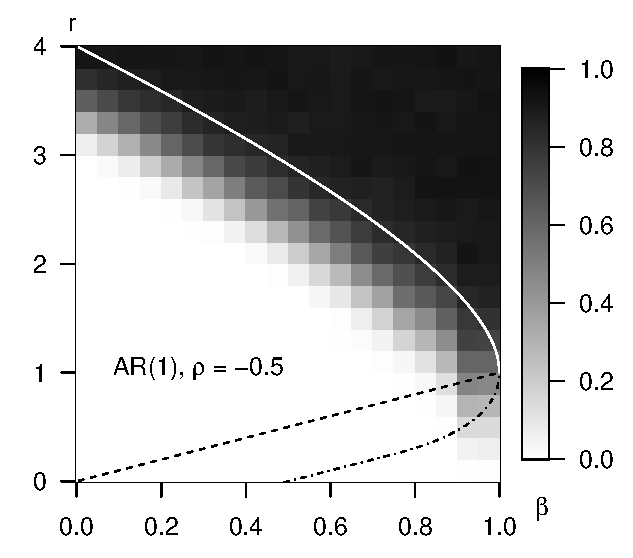
\includegraphics[width=0.4\textwidth]{./figures/simulated_phase_diagram_AR-05_p10000.eps}
    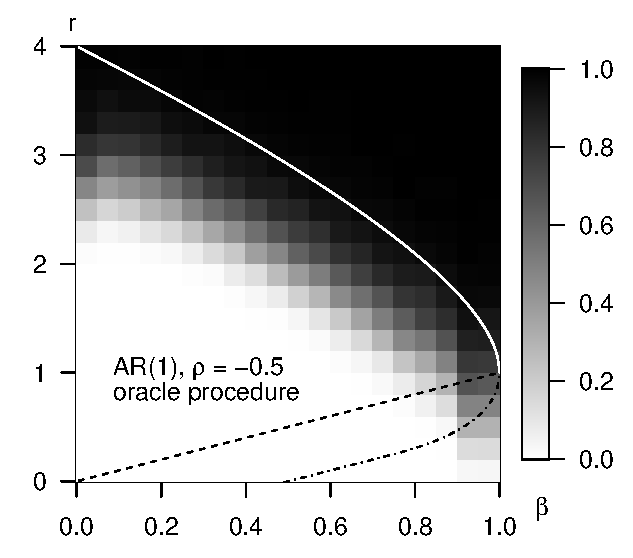
\includegraphics[width=0.4\textwidth]{./figures/simulated_phase_diagram_AR-05_p10000_oracle.eps}
    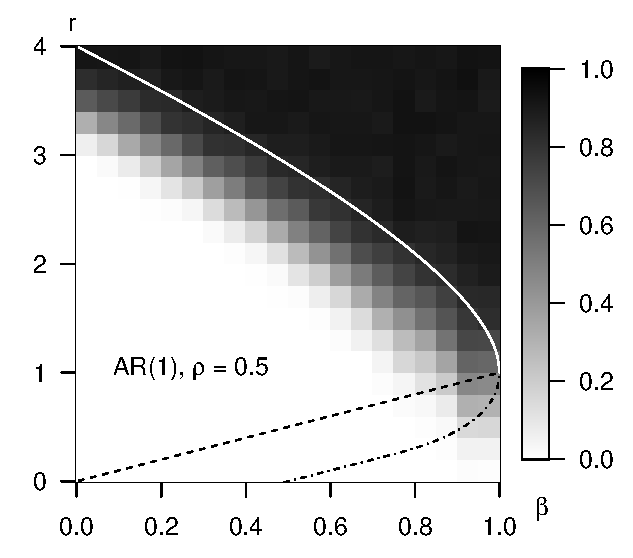
\includegraphics[width=0.4\textwidth]{./figures/simulated_phase_diagram_AR05_p10000.eps}
    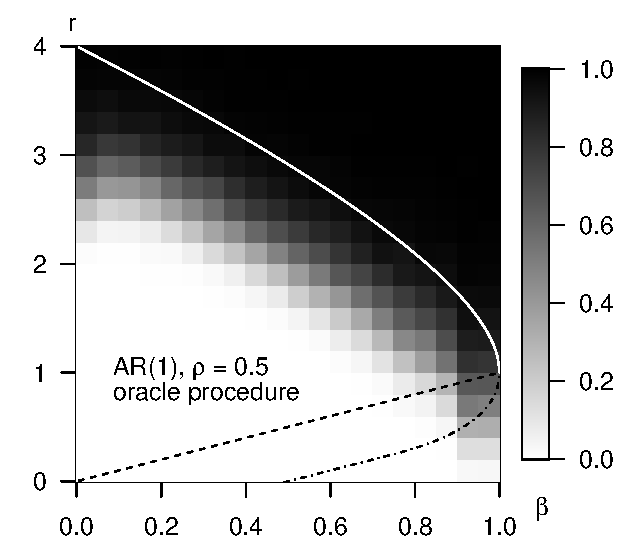
\includegraphics[width=0.4\textwidth]{./figures/simulated_phase_diagram_AR05_p10000_oracle.eps}
    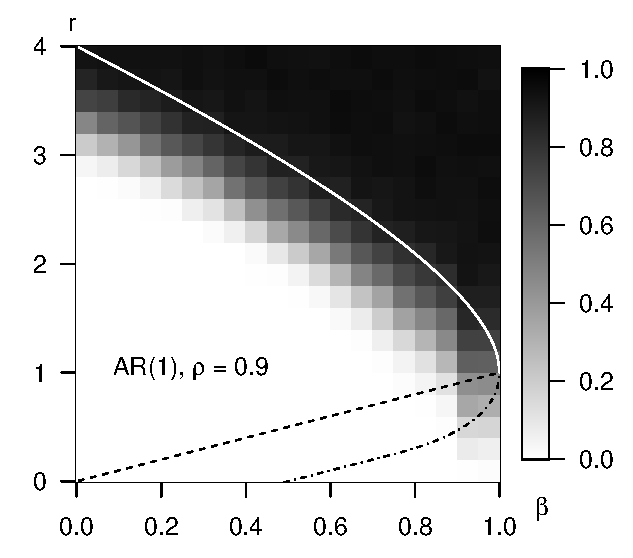
\includegraphics[width=0.4\textwidth]{./figures/simulated_phase_diagram_AR09_p10000.eps}
    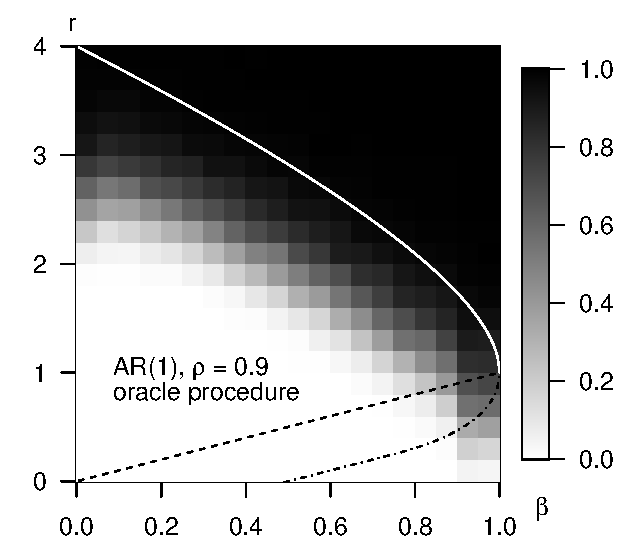
\includegraphics[width=0.4\textwidth]{./figures/simulated_phase_diagram_AR09_p10000_oracle.eps}
    \caption{The empirical probability of exact support recovery from numerical experiments, as a function of sparsity level $\beta$ and signal sizes $r$. Darker colors indicate higher probability of exact support recovery. 
    Three AR(1) models with autocorrelation functions $(-0.5)^k$ (upper), 
    $0.5^k$ (middle), and $0.9^k$ (lower) are simulated.
    The experiments were repeated 1000 times for each sparsity-signal size combination.
    In finite dimensions ($p=10000$), the Bonferroni procedures (left) suffers small loss of power compared to the oracle procedures (right).
    A phase transition in agreement with the predicted boundary \eqref{eq:strong-classification-boundary} can be seen in the AR models.
    The boundaries (solid, dashed, and dash-dotted lines) are as in Fig \ref{fig:phase-simulated}.}
    \label{fig:phase-simulated-dependent}
\end{figure}

\medskip

The second set of experiments explores exact support recovery in additive error models in the cases of long-range dependent but UDD, as well as non-UDD errors.
In particular we simulate
\begin{itemize}
    \item Fractional Gaussian noise (fGn) with Hurst parameter $H = 0.75$ and $H = 0.9$. 
    The autocovariance functions are 
    % $$\rho_{k} \sim 2H(2H-1)k^{2H-2},$$
    $$\rho_{k} \sim 0.75k^{-0.6} \quad \text{and} \quad \rho_{k} \sim 1.44k^{-0.2},$$
    as $k\to\infty$.
    Both fGn models represent the regime of long-range dependence, where covariances decay very slowly to zero, so that $\sum|\rho_k| = \infty$; see, e.g., \citep{taqqu2003livre}.
    Observe that every stationary Gaussian process with vanishing autocovariance gives rise to an UDD array as concluded in Corollary \ref{cor:stationary-Gaussian-errors}.
    \item The non-UDD Gaussian errors described in Example \ref{exmp:counter-example}.
\end{itemize}
We will apply both the sparsity-and-signal-size-agnostic Bonferroni's procedure, i.e., $\widetilde{S} = \{i:x(i)>\sqrt{2\log{p}}\}$, as well as the oracle procedure $\widehat{S}^* = \{i:x(i)\ge x_{[s]}\}$, $s=|S|$, to all settings.
Results of the numerical experiments for the fGn and non-UDD models are shown in Figure \ref{fig:phase-simulated-very-dependent}.


\begin{figure}
    \centering
    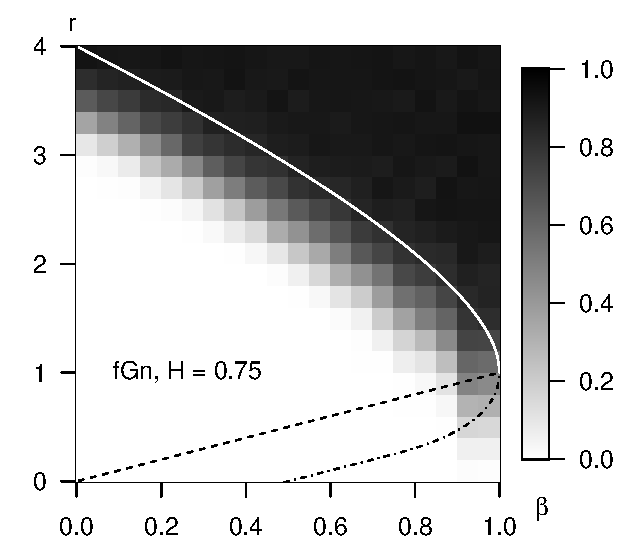
\includegraphics[width=0.4\textwidth]{./figures/simulated_phase_diagram_fGn075_p10000.eps}
    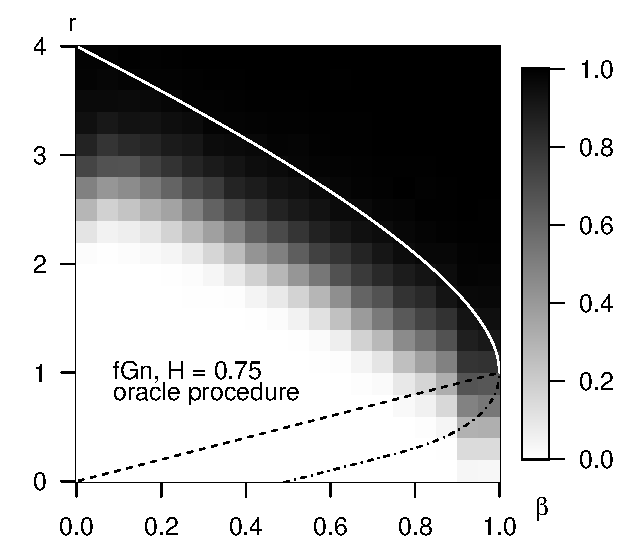
\includegraphics[width=0.4\textwidth]{./figures/simulated_phase_diagram_fGn075_p10000_oracle.eps}
    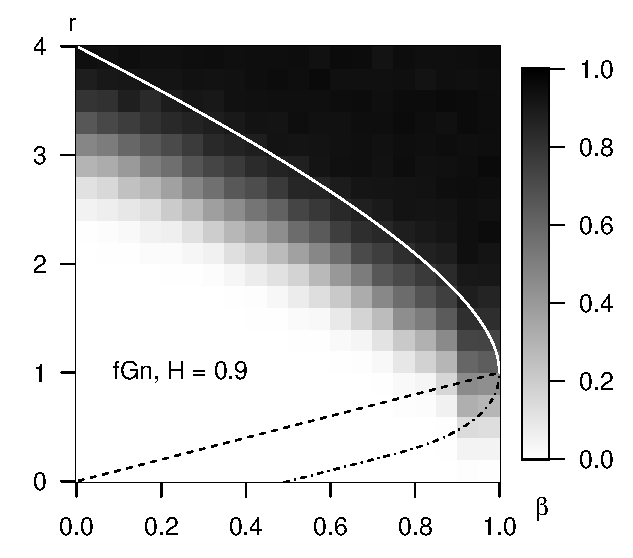
\includegraphics[width=0.4\textwidth]{./figures/simulated_phase_diagram_fGn09_p10000.eps}
    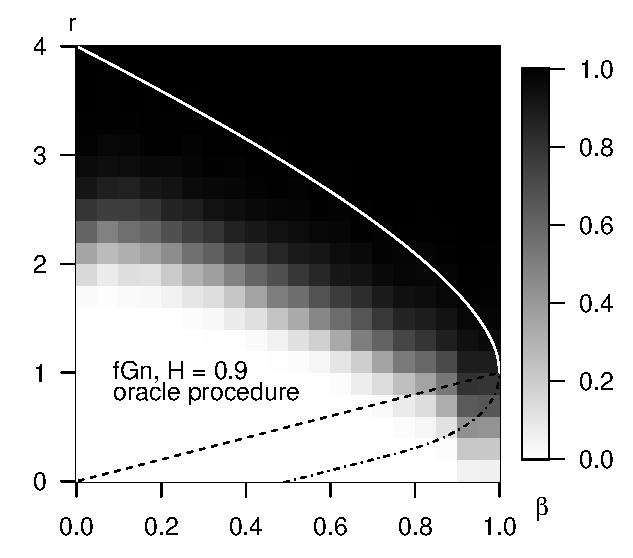
\includegraphics[width=0.4\textwidth]{./figures/simulated_phase_diagram_fGn09_p10000_oracle.eps}
    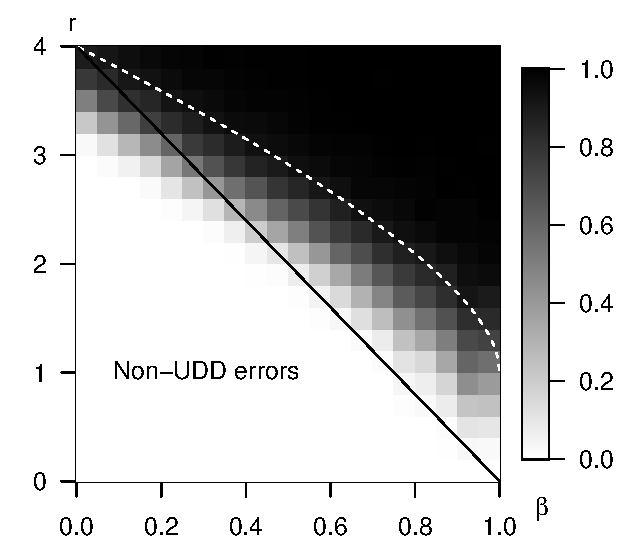
\includegraphics[width=0.4\textwidth]{./figures/simulated_phase_diagram_block_structure_p10000_agnostic7.eps}
    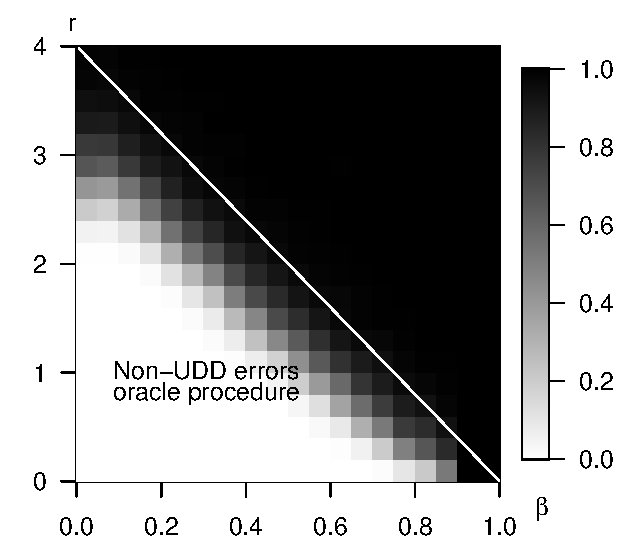
\includegraphics[width=0.4\textwidth]{./figures/simulated_phase_diagram_block_structure_p10000_oracle6.eps}
    \caption{The empirical probability of exact support recovery from numerical experiments, as a function of sparsity level $\beta$ and signal sizes $r$. Darker colors indicate higher probability of exact support recovery. 
    Two fGn models with Hurst parameter $H = 0.75$ (upper), 
    $H = 0.9$ (middle), and the non-UDD errors in Example \ref{exmp:counter-example} (lower) are simulated.
    The experiments were repeated 1000 times for each sparsity-signal size combination.
    In finite dimensions ($p=10000$), the oracle procedures (right) is able to recover support for weaker signals than the Bonferroni procedures (left) when errors are heavily dependent, although they have the same phase transition limit.
    The non-UDD errors demonstrate qualitatively different behavior, enabling support recovery for strictly weaker signals.
    The boundaries (solid, dashed, and dash-dotted lines) are as in Fig \ref{fig:phase-simulated}.
    In the non-UDD example, dashed lines represent the limit attained by Bonferroni's procedures.
    See text for additional comments.}
    \label{fig:phase-simulated-very-dependent}
\end{figure}


Notice that the oracle procedure sets its thresholds more aggressively (at roughly $\sqrt{2\log s}$) than the Bonferroni procedure (at $\sqrt{2\log p}$).
Although this difference vanishes as $p\to\infty$, in finite dimensions ($p=10\,000$) the advantage can be felt. 
Indeed, in all our experiments the oracle procedure is able to recover support of signals with higher probability than the Bonferroni procedures; compare left and right columns of Figure  \ref{fig:phase-simulated-very-dependent}.
Notice also that there is an increase in probability of recovery near $\beta=0$ for oracle procedures.
This is an artifact in finite dimensions due to the fact that $s = \lfloor p^{1-\beta}\rfloor < p/2$, and there are more signals than nulls. The oracle procedures is able to adjust to this reversal by lowering its threshold accordingly.

For UDD errors, Theorem \ref{thm:necessary} predicts that exact recovery of the support is impossible when signal sizes are below the boundary \eqref{eq:strong-classification-boundary}, even with oracle procedures. 
% Both the AR and the fGn models generate UDD Gaussian errors, and should demonstrate the same phase-transition boundary.
However, the rate of this convergence (i.e., $\P[\widehat{S}^*=S]\to0\;\text{or}\;1$) can be very slow when the errors are heavily dependent,
even though all AR and fGn models demonstrate qualitatively the same behavior in line with the predicted boundary \eqref{eq:strong-classification-boundary}. 
In finite dimensions ($p=10\,000$), as dependence in the errors increases (fGN(H=0.75) to fGN(H=0.9)), the oracle procedure becomes more powerful at recovering signal support with high probability for weaker signals. 

On the other hand, as demonstrated in Example \ref{exmp:counter-example}, non-UDD errors yield qualitatively different behavior; exact support recovery is possible for signal sizes strictly weaker than that in the UDD case. 
Lower-right panel of Figure \ref{fig:phase-simulated-very-dependent} demonstrates in this example that the signal support can be recovered as long as the signal sizes are larger than $4(1-\beta)$.


